\documentclass[aspectratio=169,10pt]{beamer}

\usepackage[T1]{fontenc}
\usepackage[utf8]{inputenc}
\usepackage{lmodern}
\usepackage{microtype}
\usepackage{amsmath}
\usepackage{booktabs}
\usepackage{array}
\usepackage{graphicx}
\usepackage{fancyvrb}
\usepackage{pgfplots}
\pgfplotsset{compat=1.18}
\usetikzlibrary{arrows.meta,positioning,calc}

\graphicspath{{./}{docs/slides/}}

% Palette sampled from the presentation in this folder.
\definecolor{burgundy}{HTML}{990000}
\definecolor{darkburgundy}{HTML}{59000E}
\definecolor{dustyrose}{HTML}{D1545B}
\definecolor{palerose}{HTML}{E5D5D6}
\definecolor{paper}{HTML}{F7F6F2}
\definecolor{softgray}{HTML}{ECEAE7}
\definecolor{midgray}{HTML}{77736F}
\definecolor{charcoal}{HTML}{434343}
\definecolor{ink}{HTML}{111111}

\setbeamercolor{normal text}{fg=ink,bg=paper}
\setbeamercolor{structure}{fg=burgundy}
\setbeamercolor{frametitle}{fg=ink,bg=paper}
\setbeamercolor{title}{fg=white}
\setbeamercolor{subtitle}{fg=palerose}
\setbeamercolor{block title}{fg=white,bg=darkburgundy}
\setbeamercolor{block body}{fg=ink,bg=softgray}
\setbeamercolor{exampleblock title}{fg=white,bg=burgundy}
\setbeamercolor{exampleblock body}{fg=ink,bg=palerose!62!paper}
\setbeamercolor{alertblock title}{fg=white,bg=charcoal}
\setbeamercolor{alertblock body}{fg=ink,bg=softgray}
\setbeamercolor{ascii body}{fg=palerose,bg=ink}

\setbeamerfont{title}{series=\bfseries,size=\Huge}
\setbeamerfont{subtitle}{size=\large}
\setbeamerfont{frametitle}{series=\bfseries,size=\Large}
\setbeamerfont{footline}{size=\scriptsize}
\setbeamertemplate{navigation symbols}{}
\setbeamertemplate{itemize item}{\color{burgundy}$\blacktriangleright$}
\setbeamertemplate{itemize subitem}{\color{dustyrose}$\bullet$}
\setbeamertemplate{caption}{\raggedright\insertcaption\par}
\setbeamertemplate{frametitle}{%
  \vspace{0.18cm}%
  \hspace{0.42cm}\insertframetitle\par
  \vspace{-0.12cm}%
  \hspace{0.42cm}{\color{burgundy}\rule{14.95cm}{0.6pt}}%
}
\setbeamertemplate{footline}{%
  \leavevmode%
  \hbox{%
    \begin{beamercolorbox}[wd=.83\paperwidth,ht=2.8ex,dp=1.1ex,leftskip=1em]{author in head/foot}%
      \color{charcoal}\insertsectionhead
    \end{beamercolorbox}%
    \begin{beamercolorbox}[wd=.17\paperwidth,ht=2.8ex,dp=1.1ex,rightskip=1em plus1fil]{date in head/foot}%
      \color{burgundy}\hfill\insertframenumber
    \end{beamercolorbox}%
  }%
}

\setlength{\tabcolsep}{5pt}
\renewcommand{\arraystretch}{1.18}

\newcommand{\projectname}{LM-IDNet}
\newcommand{\workingbadge}{%
  \colorbox{burgundy!13}{\color{darkburgundy}\scriptsize\bfseries\strut WORKING}}
\newcommand{\experimentalbadge}{%
  \colorbox{charcoal!13}{\color{charcoal}\scriptsize\bfseries\strut EXPERIMENTAL}}
\newcommand{\openbadge}{%
  \colorbox{dustyrose!18}{\color{burgundy}\scriptsize\bfseries\strut OPEN}}
\DefineVerbatimEnvironment{asciiart}{Verbatim}{
  fontsize=\small,
  baselinestretch=0.90,
  frame=none,
  fillcolor=\color{softgray},
  formatcom=\color{darkburgundy}
}

\tikzset{
  flowbox/.style={
    draw=burgundy,
    line width=0.7pt,
    rounded corners=1pt,
    fill=paper,
    minimum height=1.0cm,
    text width=2.35cm,
    align=center,
    font=\small\bfseries
  },
  smallflow/.style={
    draw=charcoal,
    rounded corners=1pt,
    fill=softgray,
    minimum height=0.78cm,
    text width=1.85cm,
    align=center,
    font=\scriptsize\bfseries
  },
  flowarrow/.style={-{Latex[length=2.2mm]},thick,draw=charcoal}
}

\title[LM-IDNet]{LM-IDNet}
\subtitle{Adaptive Dirichlet--Multinomial Anomaly Detection for IoT Traffic}
\author{Fatemeh Mahvari}
\institute{Supervisor: Professor Mauro Migliardi}
\date{9 September 2026}

\begin{document}

\begin{frame}[plain]
\begin{tikzpicture}[remember picture,overlay]
  \fill[ink] (current page.south west) rectangle (current page.north east);
  \fill[darkburgundy]
    (current page.south west) rectangle
    ([xshift=.64\paperwidth]current page.north west);
  \fill[burgundy,opacity=.28]
    ([xshift=.58\paperwidth]current page.south west) rectangle
    ([xshift=.67\paperwidth]current page.north west);
  \node[anchor=east,inner sep=0pt] (detector)
    at ([xshift=-0.42cm]current page.east)
    {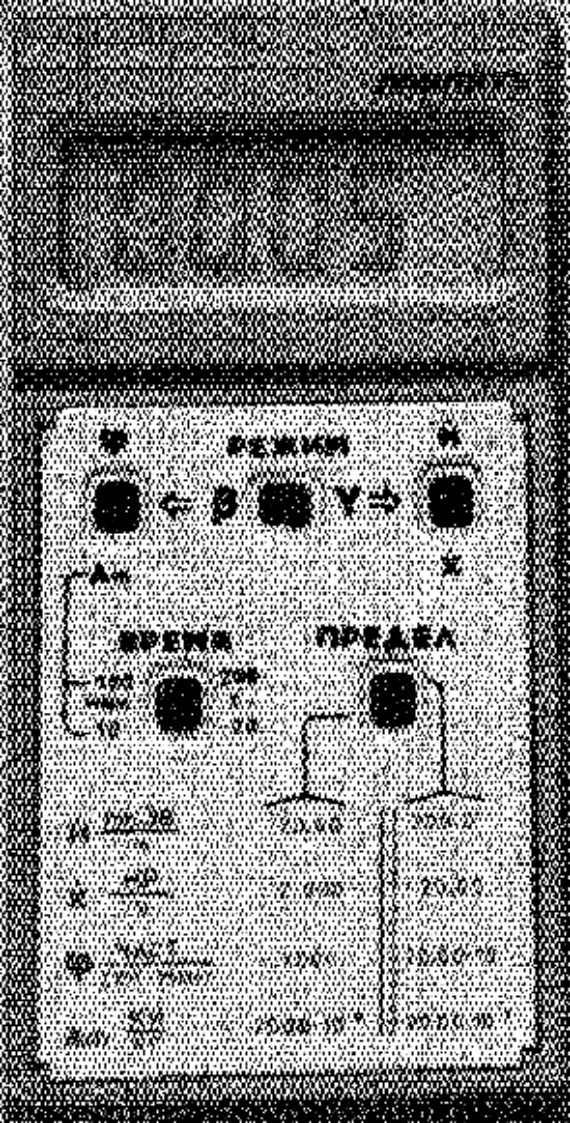
\includegraphics[height=.91\paperheight]{anomaly_detector.png}};
  \draw[palerose,line width=0.8pt]
    ([xshift=-0.10cm,yshift=0.10cm]detector.north west) rectangle
    ([xshift=0.10cm,yshift=-0.10cm]detector.south east);
  \draw[dustyrose,line width=1.1pt]
    ([xshift=-0.28cm]detector.center) -- ([xshift=0.28cm]detector.center);
  \draw[dustyrose,line width=1.1pt]
    ([yshift=-0.28cm]detector.center) -- ([yshift=0.28cm]detector.center);
  \node[anchor=west,text width=.53\paperwidth]
    at ([xshift=.70cm,yshift=.95cm]current page.west)
    {\color{white}\fontsize{28}{31}\selectfont\bfseries LM-IDNet};
  \node[anchor=west,text width=.51\paperwidth]
    at ([xshift=.72cm,yshift=-.05cm]current page.west)
    {\color{palerose}\large Adaptive Dirichlet--Multinomial\\
     Anomaly Detection for IoT Traffic};
  \node[anchor=west]
    at ([xshift=.72cm,yshift=-1.42cm]current page.west)
    {\color{white!82}\ttfamily\small [ COUNT / MODEL / DETECT / ADAPT ]};
  \node[anchor=west,text width=.50\paperwidth]
    at ([xshift=.72cm,yshift=-2.35cm]current page.west)
    {\color{palerose!90}\small Working system, experimental evidence,\\
     and the route to a defensible final evaluation};
  \node[anchor=south west,text width=.53\paperwidth]
    at ([xshift=.72cm,yshift=.40cm]current page.south west)
    {\color{white}\small\bfseries Fatemeh Mahvari\\[-0.02cm]
     \color{palerose!90}\scriptsize Supervisor: Professor Mauro Migliardi
     \quad // \quad 9 September 2026};
  \node[anchor=south east,fill=ink,fill opacity=.82,text opacity=1,
        inner xsep=3pt,inner ysep=2pt]
    at ([xshift=-.06cm,yshift=.06cm]detector.south east)
    {\color{palerose!85}\tiny REFERENCE IMAGE // PRYPIAT DETECTOR};
  \node[anchor=south east]
    at ([xshift=-.18cm,yshift=.15cm]current page.south east)
    {\color{palerose}\scriptsize\insertframenumber};
\end{tikzpicture}
\end{frame}

\section{Executive Summary}

\begin{frame}{Presentation map}
\begin{columns}[T,onlytextwidth]
\column{0.48\textwidth}
\begin{block}{From problem to working system}
\begin{enumerate}
  \item Executive summary
  \item Research problem and scientific basis
  \item Implementation work completed
  \item Datasets and experimental protocol
\end{enumerate}
\end{block}

\column{0.48\textwidth}
\begin{block}{From evidence to conclusion}
\begin{enumerate}
\setcounter{enumi}{4}
  \item Results from the working system
  \item Temporal evaluation improvements
  \item Additional detector experiments
  \item Interpretation, completion plan, and conclusion
\end{enumerate}
\end{block}
\end{columns}
\end{frame}

\begin{frame}[fragile]{Executive Summary: What the Project Is}
\begin{columns}[T,onlytextwidth]
\column{0.54\textwidth}
\projectname{} learns the ordinary network behaviour of one IoT device without
using attack examples during training.

\vspace{0.35cm}
\begin{itemize}
  \item Traffic becomes counts of TCP, ordinary UDP, SSDP, and ARP packets.
  \item A Dirichlet--multinomial model represents the expected mixture and its
  natural variability.
  \item A separately calibrated lower-tail threshold turns likelihood into an
  anomaly decision.
  \item Static and adaptive systems share the same scoring path.
\end{itemize}

\column{0.42\textwidth}
\begin{asciiart}
+--------+     +---------+
|  PCAP  | --> | WINDOWS |
+--------+     +---------+
                    |
                    v
+--------+     +---------+
| ALERTS | <-- |  MODEL  |
+--------+     +---------+
     |              |
     +----> AUDIT <-+
\end{asciiart}
\end{columns}
\end{frame}

\begin{frame}{Executive Summary: Current Project Position}
\begin{columns}[T,onlytextwidth]
\column{0.32\textwidth}
\begin{exampleblock}{\workingbadge\ Reference system}
\small
Validated capture processing, model fitting, calibration, static scoring,
labelled development evaluation, explanations, and two adaptive modes.
\end{exampleblock}

\column{0.32\textwidth}
\begin{block}{\experimentalbadge\ Additional evidence}
\small
Actual-timestamp validation, expanding temporal folds, episode metrics, and a
six-signal detector study across additional data.
\end{block}

\column{0.32\textwidth}
\begin{alertblock}{\openbadge\ Final claims}
\small
Integrated temporal validation, stronger adaptation guards, a frozen detector,
an untouched test, and measurement on intended edge hardware.
\end{alertblock}
\end{columns}

\end{frame}

\section{Research Problem and Scientific Basis}

\begin{frame}[fragile]{Research Problem: Normal IoT Traffic Changes}
\begin{columns}[T,onlytextwidth]
\column{0.55\textwidth}
\begin{itemize}
  \item IoT devices are continuously connected but often have limited compute.
  \item Signatures do not cover new attacks, failures, or misconfiguration.
  \item Ordinary traffic drifts with routines, firmware, services, and network
  conditions.
\end{itemize}

\vspace{0.35cm}
\begin{alertblock}{The design tension}
A detector must notice unusual behaviour without treating every benign change
as an attack---or absorbing an attack as the new normal.
\end{alertblock}

\column{0.41\textwidth}
\begin{asciiart}
NORMAL   ......./\...../\....
DRIFT    ...../---\../--\....
ATTACK   ..../########\.......

          LOW SCORE
              |
              v
          [  ALERT  ]
\end{asciiart}
\end{columns}
\end{frame}

\begin{frame}[fragile]{Scientific Basis: Traffic as Counts}
\begin{columns}[c,onlytextwidth]
\column{0.43\textwidth}
\begin{asciiart}
TCP    |###########|
UDP    |######     |
SSDP   |##         |
ARP    |####       |

       ONE DEVICE
       ONE WINDOW
\end{asciiart}

\column{0.53\textwidth}
For each 10-minute window:
\[
\mathbf{x}=(x_{\mathrm{TCP}},x_{\mathrm{UDP}},
x_{\mathrm{SSDP}},x_{\mathrm{ARP}}),
\qquad N=\sum_k x_k
\]

\begin{itemize}
  \item Categories are mutually exclusive; SSDP is separated from ordinary UDP.
  \item The representation is compact enough for an edge-oriented detector.
  \item Each decision retains protocol-level evidence an operator can inspect.
  \item Silence is a valid zero vector; missing capture coverage is excluded.
\end{itemize}
\end{columns}
\end{frame}

\begin{frame}{Scientific Basis: Dirichlet--Multinomial Model}
\begin{columns}[T,onlytextwidth]
\column{0.49\textwidth}
\begin{block}{Why not a fixed multinomial?}
It assumes one unchanging protocol-probability vector. Ordinary bursts and
operating modes can then appear impossible.
\end{block}

\begin{exampleblock}{Overdispersion}
\[
E[p_k]=\frac{\alpha_k}{\alpha_0},
\qquad
\alpha_0=\sum_k\alpha_k,
\qquad
\psi=\frac{1}{\alpha_0}
\]
The ratios describe the expected mixture; concentration describes how tightly
windows remain around it.
\end{exampleblock}

\column{0.47\textwidth}
\begin{block}{Decision score}
\small
\[
\begin{aligned}
\log P(\mathbf{x}\mid\boldsymbol{\alpha})
={}&\log\frac{N!}{\prod_k x_k!}
+\log\frac{\Gamma(\alpha_0)}{\Gamma(\alpha_0+N)}\\
&+\sum_k\log\frac{\Gamma(\alpha_k+x_k)}{\Gamma(\alpha_k)}
\end{aligned}
\]
\[
\text{alert if }\log P(\mathbf{x}\mid\boldsymbol{\alpha})<\tau
\]
\end{block}

\small The reported experiments use raw scores and a one-percent benign
calibration quantile.
\end{columns}
\end{frame}

\begin{frame}{Scientific Basis: Specialised Likelihood Method}
\begin{columns}[T,onlytextwidth]
\column{0.53\textwidth}
\begin{block}{Its role}
The Languasco--Migliardi method evaluates close log-Gamma differences inside
the Dirichlet--multinomial likelihood. Minka's fixed-point equations estimate
the model parameters.
\end{block}

\begin{itemize}
  \item Native code provides the production likelihood backend.
  \item SciPy remains an independent numerical reference.
  \item The D-Link workload connects the implementation to the supplied IoT
  study.
\end{itemize}

\column{0.43\textwidth}
\begin{alertblock}{Claim boundary}
A numerical backend can change runtime and numerical behaviour. It does not,
by itself, make an unchanged statistical detector more accurate.
\end{alertblock}

\begin{exampleblock}{Why D-Link is not a detection result}
Its captures provide the matched numerical workload, but the repository has no
attack ground truth for measured precision, recall, or F1.
\end{exampleblock}
\end{columns}
\end{frame}

\section{Implementation Work Completed}

\begin{frame}{Implementation: Working System Architecture}
\centering
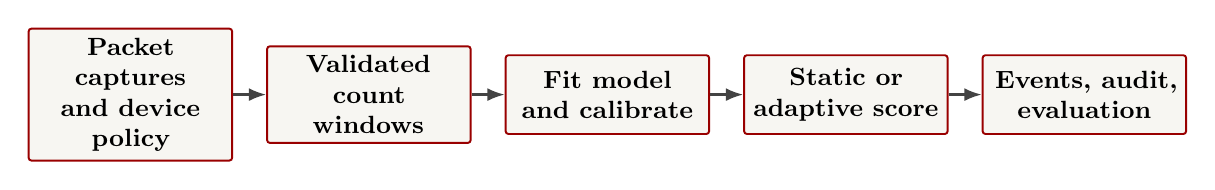
\begin{tikzpicture}[node distance=0.42cm]
\node[flowbox] (pcap) {Packet captures\\and device policy};
\node[flowbox,right=of pcap] (windows) {Validated\\count windows};
\node[flowbox,right=of windows] (fit) {Fit model\\and calibrate};
\node[flowbox,right=of fit] (score) {Static or\\adaptive score};
\node[flowbox,right=of score] (eval) {Events, audit,\\evaluation};
\draw[flowarrow] (pcap) -- (windows);
\draw[flowarrow] (windows) -- (fit);
\draw[flowarrow] (fit) -- (score);
\draw[flowarrow] (score) -- (eval);
\end{tikzpicture}

\vspace{0.55cm}
\begin{columns}[T,onlytextwidth]
\column{0.31\textwidth}
\begin{block}{Configuration}
Device identity, protocol order, data roles, estimator, backend, calibration,
adaptation mode, and random seed.
\end{block}

\column{0.31\textwidth}
\begin{block}{Artefacts}
Validated JSON models, thresholds, events, manifests, evaluations, and update
audits.
\end{block}

\column{0.31\textwidth}
\begin{block}{Operation}
One command per stage, dry-run support, stable errors, UTC logs, and isolated
experiment outputs.
\end{block}
\end{columns}
\end{frame}

\begin{frame}[fragile]{Implementation: Configuration and Controls}
\begin{columns}[T,onlytextwidth]
\column{0.48\textwidth}
\begin{exampleblock}{Configuration fails early}
Strict schemas reject unknown fields, reversed partitions, inconsistent category
counts, duplicate capture roles, invalid quantiles, and impossible buffer sizes.
\end{exampleblock}

\begin{block}{Artefacts remain compatible}
Dataset and model fingerprints stop outputs from different runs being combined
because their filenames merely look similar.
\end{block}

\column{0.48\textwidth}
\begin{asciiart}
[01] CONFIG ........ VALID
[02] DATA .......... MATCHED
[03] MODEL ......... BOUND
[04] THRESHOLD ..... ARMED
[05] STREAM ........ ACTIVE
[06] AUDIT ......... WRITTEN
\end{asciiart}

\vspace{0.3cm}
\small The shell runner selects reviewed configuration files; experiments do
not require detector source edits.
\end{columns}
\end{frame}

\begin{frame}{Implementation: Capture Processing}
\begin{columns}[T,onlytextwidth]
\column{0.54\textwidth}
\begin{itemize}
  \item Inventory, full-read validation, and policy-aware fingerprints precede
  modelling.
  \item Ethernet and ARP addresses isolate the selected device before expensive
  packet decoding.
  \item Retained packets are classified once and placed in UTC-aligned,
  half-open windows.
  \item Complete silence and missing recording coverage remain distinct states.
  \item Labels are separate, time-aligned records joined only for evaluation.
\end{itemize}

\column{0.42\textwidth}
\begin{exampleblock}{Measured preprocessing gain}
\centering
\Huge\textbf{280.0 s $\rightarrow$ 12.5 s}\\[0.15cm]
\small 1.48 GB mixed-device capture\\
byte-identical processed JSON
\end{exampleblock}

\begin{alertblock}{Provenance retained}
Capture IDs, hashes, time ranges, excluded files, incomplete days, labels, and
partition roles remain auditable.
\end{alertblock}
\end{columns}
\end{frame}

\begin{frame}{Implementation: Fit, Calibrate, Score, Explain, Evaluate}
\begin{columns}[T,onlytextwidth]
\column{0.58\textwidth}
\centering
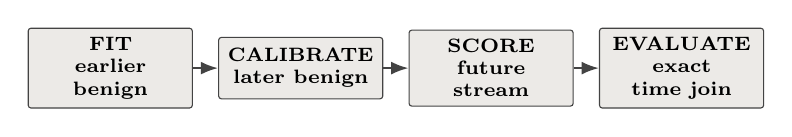
\begin{tikzpicture}[node distance=0.32cm]
\node[smallflow] (fit) {FIT\\earlier benign};
\node[smallflow,right=of fit] (cal) {CALIBRATE\\later benign};
\node[smallflow,right=of cal] (score) {SCORE\\future stream};
\node[smallflow,right=of score] (eval) {EVALUATE\\exact time join};
\draw[flowarrow] (fit) -- (cal);
\draw[flowarrow] (cal) -- (score);
\draw[flowarrow] (score) -- (eval);
\end{tikzpicture}

\vspace{0.55cm}
\begin{itemize}
  \item Fitting stores alpha, convergence, likelihood, runtime, data identity,
  and time range.
  \item Calibration stores the lower quantile, IQR, score distribution, and
  model fingerprint.
  \item Every event stores counts, score, decision, severity, expected profile,
  category residuals, and fingerprint.
\end{itemize}

\column{0.38\textwidth}
\begin{alertblock}{Interpretation boundary}
Residuals explain which categories were high or low. They do not diagnose an
attack family.
\end{alertblock}
\end{columns}
\end{frame}

\begin{frame}{Implementation: Native Likelihood Integration}
\begin{columns}[T,onlytextwidth]
\column{0.48\textwidth}
\begin{block}{Safety work}
\begin{itemize}
  \item Exact zero result for zero counts
  \item Checked coefficients, files, dimensions, and allocations
  \item Native failures returned to Python
  \item Workspaces released after success or failure
  \item Reproducible container compilation
\end{itemize}
\end{block}

\column{0.48\textwidth}
\begin{block}{Production work}
\begin{itemize}
  \item Matrix entry point for independent rows
  \item One shared setup for the complete matrix
  \item Alpha conversion and typed exceptions in the adapter
  \item Protection around legacy global state
  \item Row-wise statistical meaning preserved
\end{itemize}
\end{block}
\end{columns}

\end{frame}

\begin{frame}[fragile]{Adaptation Modes: Shared Scoring Path}
\begin{columns}[T,onlytextwidth]
\column{0.48\textwidth}
\begin{asciiart}
+---------+     +----------+
| WINDOW  | --> | SCORE IT |
+---------+     +----------+
                       |
                       v
                  +----------+
                  | RECORD   |
                  +----------+
                       |
                       v
                  UPDATE FUTURE
\end{asciiart}

\column{0.48\textwidth}
\begin{block}{Static}
Model and threshold never change.
\end{block}
\begin{block}{Adaptive threshold}
Alpha stays fixed; the recent-score quantile and IQR can change.
\end{block}
\begin{block}{Periodic refit}
A static gate admits apparently safe windows; guarded candidates can replace
future model state.
\end{block}
\end{columns}

\end{frame}

\begin{frame}{Adaptation Mode: Threshold-Only}
\begin{columns}[T,onlytextwidth]
\column{0.55\textwidth}
\begin{enumerate}
  \item Score the current non-missing window with fixed
  $\boldsymbol{\alpha}_0$.
  \item Append its score to a bounded recent-score buffer.
  \item At the configured interval, calculate the same lower quantile and IQR.
  \item Promote the new threshold only when the candidate IQR is positive.
\end{enumerate}

\column{0.41\textwidth}
\begin{alertblock}{Deliberately weak baseline}
Every recent score enters the buffer, including anomalous scores. This makes the
mode a clean test of threshold drift, not a claim of safe online learning.
\end{alertblock}

\begin{exampleblock}{What stays fixed}
Alpha, expected protocol profile, and original model fingerprint.
\end{exampleblock}
\end{columns}
\end{frame}

\begin{frame}{Adaptation Mode: Guarded Periodic Refitting}
\centering
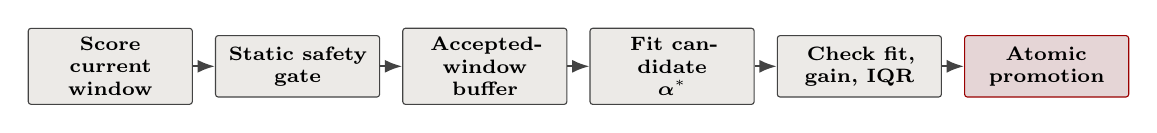
\begin{tikzpicture}[node distance=0.28cm]
\node[smallflow] (score) {Score current\\window};
\node[smallflow,right=of score] (gate) {Static safety\\gate};
\node[smallflow,right=of gate] (buffer) {Accepted-window\\buffer};
\node[smallflow,right=of buffer] (fit) {Fit candidate\\$\boldsymbol{\alpha}^{*}$};
\node[smallflow,right=of fit] (guards) {Check fit,\\gain, IQR};
\node[smallflow,right=of guards,fill=palerose,draw=burgundy] (promote) {Atomic\\promotion};
\draw[flowarrow] (score) -- (gate);
\draw[flowarrow] (gate) -- (buffer);
\draw[flowarrow] (buffer) -- (fit);
\draw[flowarrow] (fit) -- (guards);
\draw[flowarrow] (guards) -- (promote);
\end{tikzpicture}

\vspace{0.50cm}
\begin{columns}[T,onlytextwidth]
\column{0.48\textwidth}
\begin{block}{Immutable admission gate}
\[
s_0(\mathbf{x}_t)\geq
\tau_0+m\operatorname{IQR}_0
\]
The unchanged original detector judges every candidate window.
\end{block}

\column{0.48\textwidth}
\begin{block}{Fail-closed promotion}
The candidate must converge, improve accepted-buffer likelihood, and give recent
scores a positive IQR. Model, threshold, profile, and fingerprint change
together; rejection retains the old model.
\end{block}
\end{columns}

\small Four one-count smoothing rows prevent a temporarily absent protocol from
forcing an invalid zero alpha.
\end{frame}

\begin{frame}{Implementation: Validation and Generated Evidence}
\begin{columns}[T,onlytextwidth]
\column{0.45\textwidth}
\begin{exampleblock}{Automated validation boundary}
\centering
\Huge\textbf{261 passed}\\[0.18cm]
\small 10 slow, PCAP, or benchmark checks excluded by default markers
\end{exampleblock}

\column{0.51\textwidth}
\begin{itemize}
  \item Configuration, timestamps, classification, aggregation, and schemas
  \item Failure handling, fitting, calibration, scoring, and evaluation
  \item Native/reference agreement and benchmarking
  \item Adaptation ordering, candidate promotion, rejection, and fingerprints
\end{itemize}
\end{columns}

\vspace{0.35cm}
\begin{block}{Evidence is written, not inferred}
Separate experiment directories retain models, thresholds, events, evaluations,
adaptation audits, capture records, benchmarks, and UTC logs. Dry runs do not
mutate these outputs.
\end{block}
\end{frame}

\section{Datasets and Experimental Protocol}

\begin{frame}{Dataset Protocol: Roles and Composition}
\begin{columns}[T,onlytextwidth]
\column{0.31\textwidth}
\begin{block}{D-Link Camera 5}
\small
\begin{tabular}{@{}lr@{}}
Fit & 846\\
Calibration & 288\\
Development & 270\\
Final & 288\\
\end{tabular}
\par\medskip
Reference numerical workload; no attack labels in the repository.
\end{block}

\column{0.33\textwidth}
\begin{block}{UNSW Chromecast}
\small
\begin{tabular}{@{}lr@{}}
Fit & 867 (0)\\
Calibration & 576 (0)\\
Development & 474 (32)\\
Final & 432 (6)\\
\end{tabular}
\par\medskip
Parentheses show attack windows. October 24 is excluded because the source
capture is truncated.
\end{block}

\column{0.33\textwidth}
\begin{block}{UNSW Samsung camera}
\small
\begin{tabular}{@{}lr@{}}
Fit & 432 (0)\\
Calibration & 81 (0)\\
Development & 556 (70)\\
Final & 576 (12)\\
\end{tabular}
\par\medskip
Parentheses show attack windows. Captures are filtered to the selected MAC
address.
\end{block}
\end{columns}

\end{frame}

\begin{frame}[fragile]{Dataset Protocol: Chronology and Leakage}
\begin{columns}[T,onlytextwidth]
\column{0.58\textwidth}
\begin{asciiart}
PAST -----------------------> FUTURE

[ FIT ] -> [ CAL ] -> [ DEV ] -> [ SEALED ]
 benign    benign    labels       test
 history   limit     after run     data
\end{asciiart}

\column{0.38\textwidth}
\begin{itemize}
  \item Whole captures remain intact.
  \item Labels never fit alpha or thresholds.
  \item Labels never admit adaptive windows.
  \item Development labels compare completed runs.
\end{itemize}
\end{columns}

\vspace{0.35cm}
\begin{alertblock}{What capture-level chronology does not solve}
Adjacent windows remain correlated, one boundary provides only one history, and
capture names alone do not prove that processed time ranges are disjoint.
\end{alertblock}
\end{frame}

\section{Results from the Working System}

\begin{frame}{Static Result: Precision and Recall}
\begin{columns}[c,onlytextwidth]
\column{0.69\textwidth}
\centering
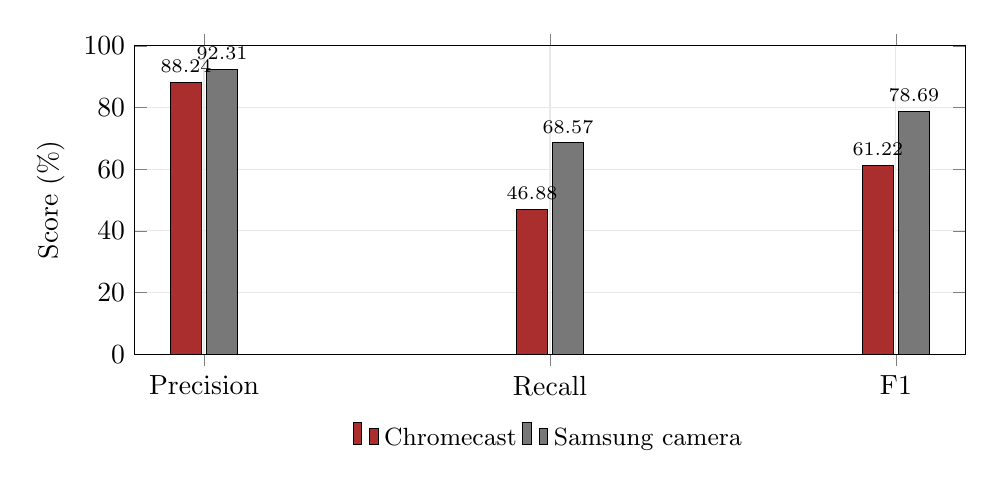
\begin{tikzpicture}
\begin{axis}[
  ybar,
  bar width=11pt,
  width=\linewidth,
  height=5.5cm,
  ymin=0,
  ymax=100,
  ylabel={Score (\%)},
  symbolic x coords={precision,recall,f1},
  xtick=data,
  xticklabels={Precision,Recall,F1},
  ytick={0,20,40,60,80,100},
  grid=major,
  grid style={gray!18},
  legend style={font=\small,draw=none,at={(0.5,-0.20)},anchor=north,legend columns=2},
  nodes near coords,
  nodes near coords style={font=\scriptsize},
]
\addplot[fill=burgundy!82] coordinates {
  (precision,88.24) (recall,46.88) (f1,61.22)
};
\addlegendentry{Chromecast}
\addplot[fill=charcoal!72] coordinates {
  (precision,92.31) (recall,68.57) (f1,78.69)
};
\addlegendentry{Samsung camera}
\end{axis}
\end{tikzpicture}

\column{0.27\textwidth}
\begin{block}{Chromecast}
\centering\small
15 TP \quad 440 TN\\
2 FP \quad 17 FN
\end{block}
\begin{block}{Samsung}
\centering\small
48 TP \quad 482 TN\\
4 FP \quad 22 FN
\end{block}
\begin{alertblock}{D-Link}
\small No labelled detection metric; used for numerical benchmarking.
\end{alertblock}
\end{columns}
\end{frame}

\begin{frame}{Adaptation Result: Mode Comparison}
\centering
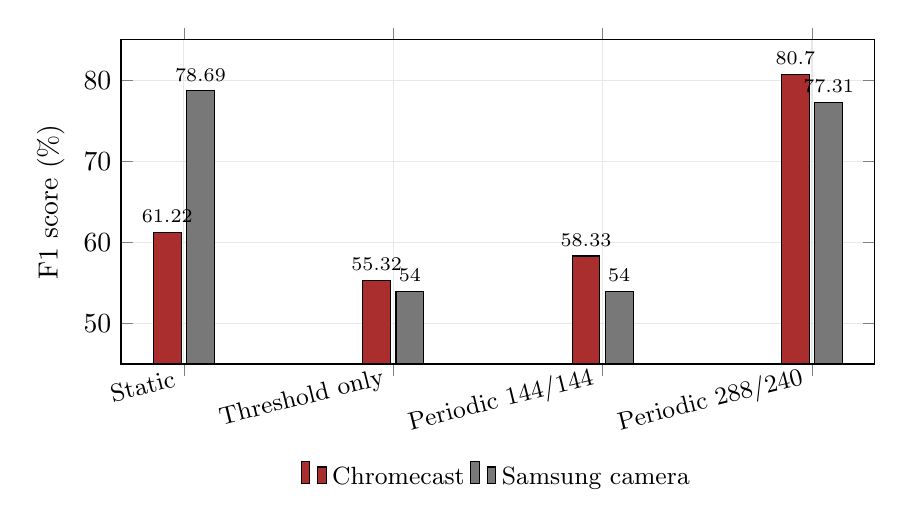
\begin{tikzpicture}
\begin{axis}[
  ybar,
  bar width=10pt,
  width=0.92\textwidth,
  height=5.7cm,
  ymin=45,
  ymax=85,
  ylabel={F1 score (\%)},
  symbolic x coords={static,threshold,periodic144,periodic288},
  xtick=data,
  xticklabels={Static,Threshold only,Periodic 144/144,Periodic 288/240},
  x tick label style={font=\small,rotate=14,anchor=east},
  grid=major,
  grid style={gray!18},
  legend style={font=\small,draw=none,at={(0.5,-0.28)},anchor=north,legend columns=2},
  nodes near coords,
  nodes near coords style={font=\scriptsize},
]
\addplot[fill=burgundy!82] coordinates {
  (static,61.22) (threshold,55.32) (periodic144,58.33) (periodic288,80.70)
};
\addlegendentry{Chromecast}
\addplot[fill=charcoal!72] coordinates {
  (static,78.69) (threshold,54.00) (periodic144,54.00) (periodic288,77.31)
};
\addlegendentry{Samsung camera}
\end{axis}
\end{tikzpicture}

\small Threshold-only adaptation worsened both devices. The selected periodic
configuration improved Chromecast and remained close to the Samsung static
baseline, but it was selected on development data.
\end{frame}

\begin{frame}{Adaptation Result: Cadence -- Chromecast}
\centering
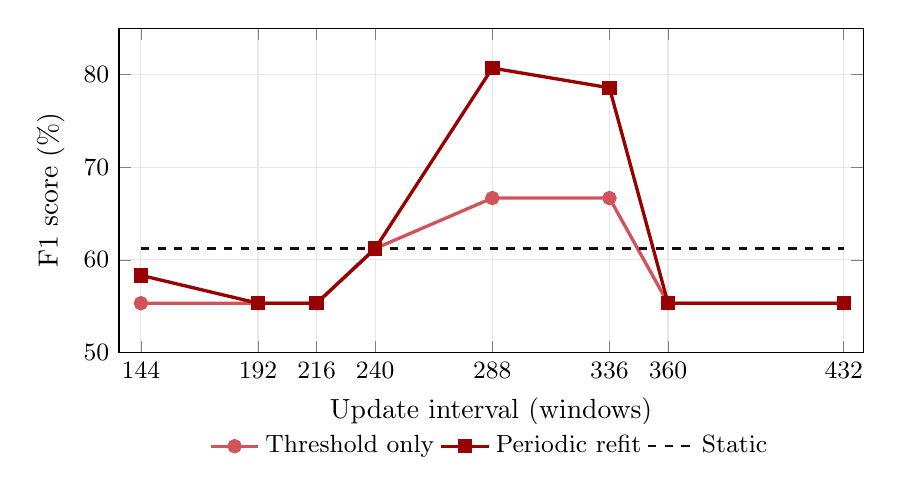
\begin{tikzpicture}
\begin{axis}[
  width=0.91\textwidth,
  height=5.7cm,
  xmin=135,
  xmax=440,
  ymin=50,
  ymax=85,
  xtick={144,192,216,240,288,336,360,432},
  x tick label style={font=\small},
  y tick label style={font=\small},
  xlabel={Update interval (windows)},
  ylabel={F1 score (\%)},
  grid=major,
  grid style={gray!18},
  legend style={font=\small,draw=none,at={(0.5,-0.22)},anchor=north,legend columns=3},
]
\addplot[color=dustyrose,very thick,mark=*] coordinates {
  (144,55.32) (192,55.32) (216,55.32) (240,61.22)
  (288,66.67) (336,66.67) (360,55.32) (432,55.32)
};
\addlegendentry{Threshold only}
\addplot[color=burgundy,very thick,mark=square*] coordinates {
  (144,58.33) (192,55.32) (216,55.32) (240,61.22)
  (288,80.70) (336,78.57) (360,55.32) (432,55.32)
};
\addlegendentry{Periodic refit}
\addplot[color=ink,dashed,thick] coordinates {(144,61.22) (432,61.22)};
\addlegendentry{Static}
\end{axis}
\end{tikzpicture}

\end{frame}

\begin{frame}{Adaptation Result: Cadence -- Samsung Camera}
\centering
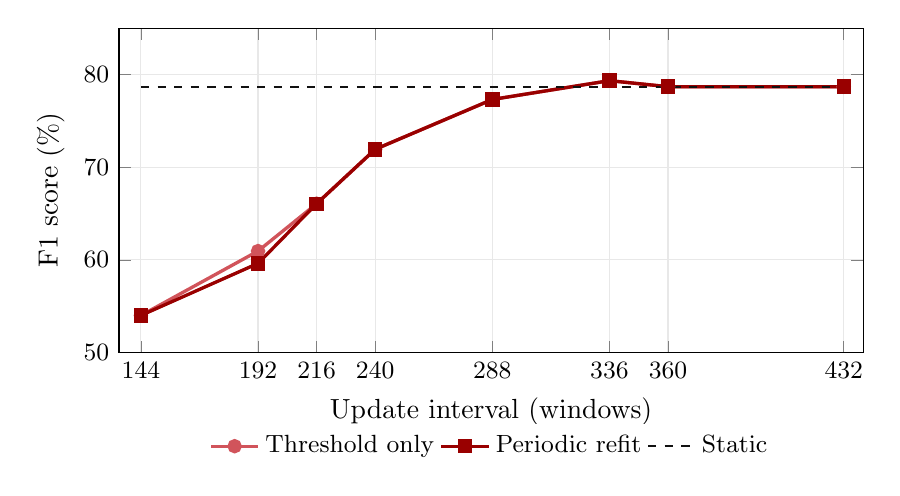
\begin{tikzpicture}
\begin{axis}[
  width=0.91\textwidth,
  height=5.7cm,
  xmin=135,
  xmax=440,
  ymin=50,
  ymax=85,
  xtick={144,192,216,240,288,336,360,432},
  x tick label style={font=\small},
  y tick label style={font=\small},
  xlabel={Update interval (windows)},
  ylabel={F1 score (\%)},
  grid=major,
  grid style={gray!18},
  legend style={font=\small,draw=none,at={(0.5,-0.22)},anchor=north,legend columns=3},
]
\addplot[color=dustyrose,very thick,mark=*] coordinates {
  (144,54.00) (192,60.95) (216,66.06) (240,71.93)
  (288,77.31) (336,79.34) (360,78.69) (432,78.69)
};
\addlegendentry{Threshold only}
\addplot[color=burgundy,very thick,mark=square*] coordinates {
  (144,54.00) (192,59.62) (216,66.06) (240,71.93)
  (288,77.31) (336,79.34) (360,78.69) (432,78.69)
};
\addlegendentry{Periodic refit}
\addplot[color=ink,dashed,thick] coordinates {(144,78.69) (432,78.69)};
\addlegendentry{Static}
\end{axis}
\end{tikzpicture}

\end{frame}

\begin{frame}{Adaptation safety: attack contamination}
\begin{columns}[c,onlytextwidth]
\column{0.72\textwidth}
\centering
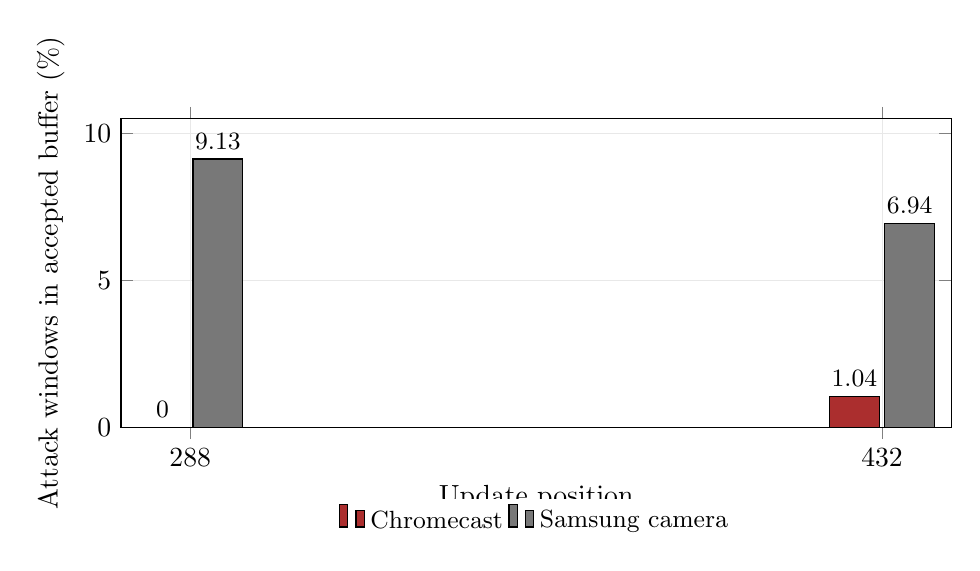
\begin{tikzpicture}
\begin{axis}[
  ybar,
  bar width=18pt,
  width=\linewidth,
  height=5.5cm,
  ymin=0,
  ymax=10.5,
  ylabel={Attack windows in accepted buffer (\%)},
  symbolic x coords={288,432},
  xtick=data,
  xlabel={Update position},
  grid=major,
  grid style={gray!18},
  legend style={font=\small,draw=none,at={(0.5,-0.23)},anchor=north,legend columns=2},
  nodes near coords,
  nodes near coords style={font=\small},
]
\addplot[fill=burgundy!82] coordinates {(288,0.00) (432,1.04)};
\addlegendentry{Chromecast}
\addplot[fill=charcoal!72] coordinates {(288,9.13) (432,6.94)};
\addlegendentry{Samsung camera}
\end{axis}
\end{tikzpicture}

\column{0.24\textwidth}
\begin{alertblock}{Observed failure}
The selected Samsung buffer contained 22 attack windows at its first update.
\end{alertblock}
\begin{block}{Implication}
A larger margin on the same composition score cannot reject attacks that already
look compositionally ordinary.
\end{block}
\end{columns}
\end{frame}

\begin{frame}{Adaptation safety: model movement}
\begin{columns}[c,onlytextwidth]
\column{0.72\textwidth}
\centering
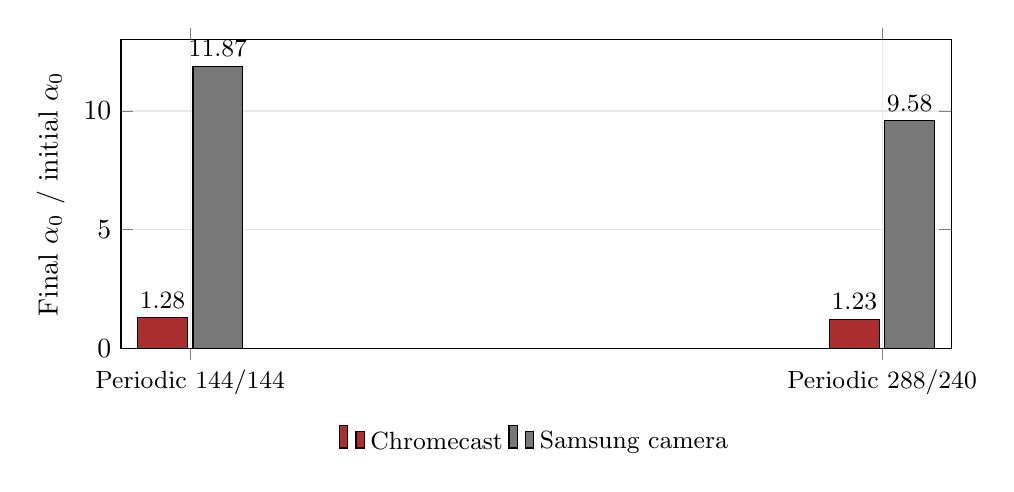
\begin{tikzpicture}
\begin{axis}[
  ybar,
  bar width=18pt,
  width=\linewidth,
  height=5.5cm,
  ymin=0,
  ymax=13,
  ylabel={Final $\alpha_0$ / initial $\alpha_0$},
  symbolic x coords={initial,selected},
  xtick=data,
  xticklabels={Periodic 144/144,Periodic 288/240},
  x tick label style={font=\small},
  grid=major,
  grid style={gray!18},
  legend style={font=\small,draw=none,at={(0.5,-0.23)},anchor=north,legend columns=2},
  nodes near coords,
  nodes near coords style={font=\small},
]
\addplot[fill=burgundy!82] coordinates {(initial,1.28) (selected,1.23)};
\addlegendentry{Chromecast}
\addplot[fill=charcoal!72] coordinates {(initial,11.87) (selected,9.58)};
\addlegendentry{Samsung camera}
\end{axis}
\end{tikzpicture}

\column{0.24\textwidth}
\begin{alertblock}{Observed failure}
Samsung concentration increased by a factor of 9.58 under the selected policy.
\end{alertblock}
\begin{block}{Next guard}
Blend old and candidate alpha, or reject excessive concentration movement.
\end{block}
\end{columns}
\end{frame}

\begin{frame}{Numerical Result: Workload-Dependent Runtime}
\begin{columns}[c,onlytextwidth]
\column{0.75\textwidth}
\centering
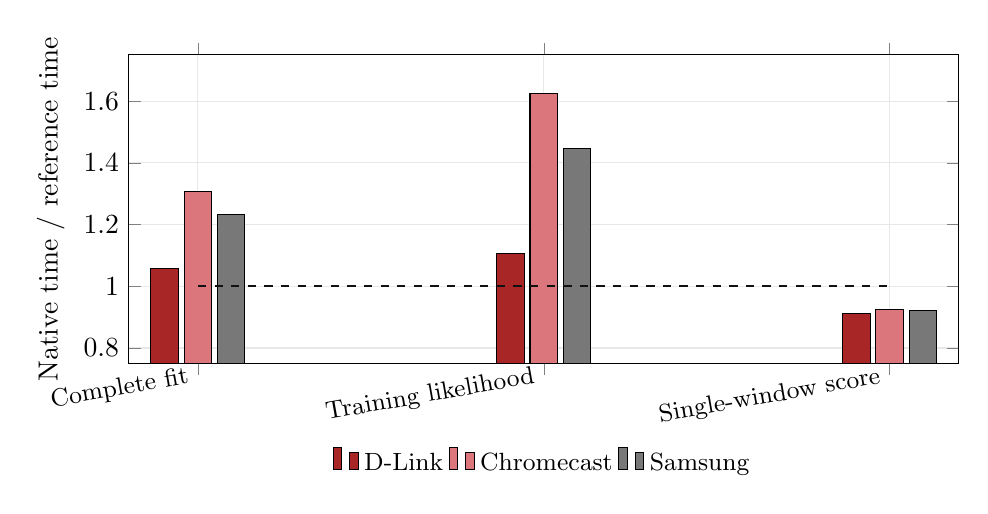
\begin{tikzpicture}
\begin{axis}[
  ybar,
  bar width=10pt,
  width=\linewidth,
  height=5.5cm,
  ymin=0.75,
  ymax=1.75,
  ylabel={Native time / reference time},
  symbolic x coords={fit,matrix,window},
  xtick=data,
  xticklabels={Complete fit,Training likelihood,Single-window score},
  x tick label style={font=\small,rotate=10,anchor=east},
  grid=major,
  grid style={gray!18},
  legend style={font=\small,draw=none,at={(0.5,-0.25)},anchor=north,legend columns=3},
]
\addplot[fill=burgundy!85] coordinates {(fit,1.058) (matrix,1.105) (window,0.911)};
\addlegendentry{D-Link}
\addplot[fill=dustyrose!80] coordinates {(fit,1.307) (matrix,1.625) (window,0.924)};
\addlegendentry{Chromecast}
\addplot[fill=charcoal!72] coordinates {(fit,1.232) (matrix,1.447) (window,0.923)};
\addlegendentry{Samsung}
\draw[ink,dashed,thick] (axis cs:fit,1) -- (axis cs:window,1);
\end{axis}
\end{tikzpicture}

\column{0.21\textwidth}
\begin{exampleblock}{Agreement}
\centering
\Large\textbf{0 / 270}\\[-0.05cm]
\small decision mismatches
\end{exampleblock}
\begin{block}{Maximum differences}
\centering\small
relative alpha\\
$3.86\times10^{-7}$\\[0.2cm]
absolute score\\
$1.09\times10^{-5}$
\end{block}
\end{columns}

\small Ratios below one are faster. The native path is slightly faster for
online single-window scoring, but slower for full fitting and matrix likelihood.
\end{frame}

\section{Temporal Evaluation Improvements}

\begin{frame}{Temporal Evaluation: Why One Split Is Not Enough}
\begin{columns}[T,onlytextwidth]
\column{0.53\textwidth}
\begin{itemize}
  \item One fit/calibration/development boundary represents only one history.
  \item Adjacent windows are correlated, so window count overstates independent
  evidence.
  \item Consecutive attack windows can be one incident rather than several.
  \item Pooled metrics can hide a poor capture or operating period.
\end{itemize}

\column{0.43\textwidth}
\begin{block}{Measured dependence}
\small
\begin{tabular}{@{}lr@{}}
Chromecast packet-count lag 1 & $\approx 0.86$\\
Chromecast score lag 1 & $\approx 0.39$\\
Samsung score lag 1 & $\approx 0.42$\\
\end{tabular}
\end{block}

\begin{alertblock}{Required reporting}
Per-capture results, attack-episode recall, false-alert episodes per day,
detection delay, and block-level uncertainty.
\end{alertblock}
\end{columns}
\end{frame}

\begin{frame}[fragile]{Temporal Evaluation: Fold Design and Evidence}
\begin{columns}[T,onlytextwidth]
\column{0.51\textwidth}
\begin{asciiart}
F1 [FIT] -> CAL -> CHECK
F2 [=== FIT ===] -> CAL -> CHECK
F3 [===== FIT =====] -> CAL -> CHECK

RULE: earlier history only; final data outside
\end{asciiart}

\vspace{0.28cm}
\small Actual UTC ranges are ordered globally; unexplained overlaps stop the
run. One D-Link fit issue contains 144 repeated window identities and must be
resolved before final fitting.

\column{0.45\textwidth}
\begin{block}{Labelled temporal folds}
\small
\begin{tabular}{@{}lrr@{}}
\toprule
& \textbf{Episode} & \textbf{False-alert}\\
\textbf{Dataset} & \textbf{recall} & \textbf{episodes/day}\\
\midrule
Chromecast & 0.70 & 0.91\\
Samsung camera & 0.82 & 0.78\\
\bottomrule
\end{tabular}
\end{block}

\begin{alertblock}{Calibration is not a guarantee}
Two benign Chromecast folds each contain 288 windows, yet produce 12 and 2 false
alerts under the same quantile rule.
\end{alertblock}
\end{columns}
\end{frame}

\section{Additional Detector Experiments}

\begin{frame}[fragile]{Detector Experiment: Composition Gap}
\begin{columns}[T,onlytextwidth]
\column{0.52\textwidth}
One missed UDP flood retained an ordinary-looking protocol proportion while
sending far more traffic. Other missed attacks changed connection attempts, ARP
activity, bytes, or direction without making the four-category mixture unlikely.

\vspace{0.35cm}
\begin{alertblock}{Representation gap}
The composition score asks, ``Is this protocol mixture normal?'' It does not ask,
``Is the amount or direction of traffic normal?''
\end{alertblock}

\column{0.44\textwidth}
\begin{asciiart}
+-------------------------+
| COMPOSITION  TCP/UDP/...|
+-------------------------+
| VOLUME       packets    |
| SIZE         bytes      |
| CONNECTION   TCP SYN    |
| LOCAL LINK   ARP        |
| DIRECTION    in / out   |
+-------------------------+
\end{asciiart}
\end{columns}
\end{frame}

\begin{frame}{Detector Experiment: Chromecast Development}
\centering
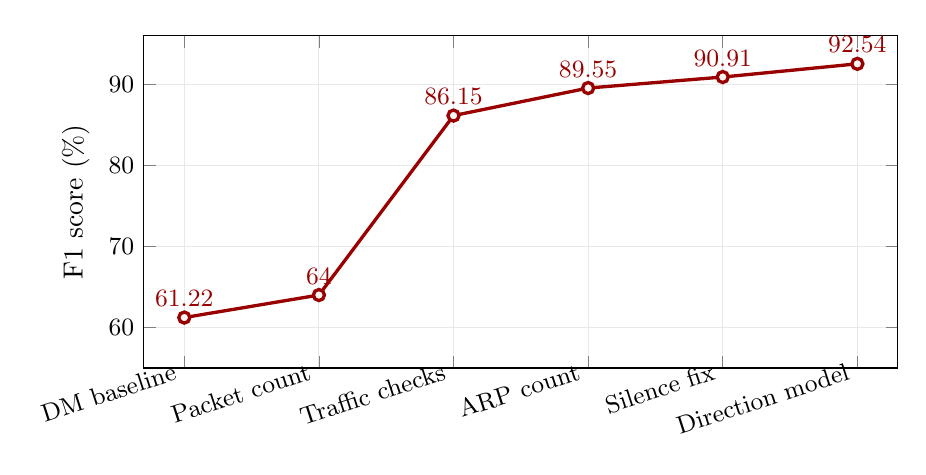
\begin{tikzpicture}
\begin{axis}[
  width=0.92\textwidth,
  height=5.8cm,
  ymin=55,
  ymax=96,
  xmin=0.7,
  xmax=6.3,
  xtick={1,2,3,4,5,6},
  xticklabels={DM baseline,Packet count,Traffic checks,ARP count,Silence fix,Direction model},
  x tick label style={font=\small,rotate=18,anchor=east},
  y tick label style={font=\small},
  ylabel={F1 score (\%)},
  grid=major,
  grid style={gray!18},
  nodes near coords,
  nodes near coords style={font=\small},
]
\addplot[color=burgundy,very thick,mark=*,mark options={fill=paper}] coordinates {
  (1,61.22) (2,64.00) (3,86.15) (4,89.55) (5,90.91) (6,92.54)
};
\end{axis}
\end{tikzpicture}

\end{frame}

\begin{frame}{Detector Experiment: Cross-Device Evidence}
\centering
\small
\begin{tabular}{@{}lrrrrr@{}}
\toprule
\textbf{Evaluation} & \textbf{TP} & \textbf{FP} & \textbf{FN} & \textbf{F1} & \textbf{ROC--AUC}\\
\midrule
Chromecast development, latest detector & 31 & 4 & 1 & 92.54\% & 99.70\%\\
Amazon Echo development, no retuning & 9 & 5 & 3 & 69.23\% & 95.93\%\\
Chromecast final, earlier frozen detector & 4 & 2 & 2 & 66.67\% & 99.77\%\\
\bottomrule
\end{tabular}

\vspace{0.45cm}
\begin{columns}[T,onlytextwidth]
\column{0.48\textwidth}
\begin{exampleblock}{What transferred}
The Echo run detected every labelled ARP attack window and showed sub-millisecond
mean scoring latency on the development host.
\end{exampleblock}

\column{0.48\textwidth}
\begin{alertblock}{What did not transfer cleanly}
Low-rate UDP attacks remained difficult, false alerts increased, and the opened
Chromecast final data cannot validate later direction or score-ranking changes.
\end{alertblock}
\end{columns}
\end{frame}

\begin{frame}{Detector Experiment: Rejected and Retained Changes}
\begin{columns}[T,onlytextwidth]
\column{0.48\textwidth}
\begin{alertblock}{Rejected after measurement}
\small
\begin{itemize}
  \item Adjacent-window byte change: extra false alerts
  \item Mean packet-size tails: unstable across devices
  \item Corroboration rules: suppressed valid single-signal attacks
  \item Automatic adaptive promotion: failed the later-traffic safety check
\end{itemize}
\end{alertblock}

\column{0.48\textwidth}
\begin{exampleblock}{Carry forward selectively}
\small
\begin{itemize}
  \item Packet, byte, TCP SYN, and ARP counts
  \item Direction model
  \item Episode metrics and detector-health report
  \item Score normalisation only if one cross-feature ranking is required
\end{itemize}
\end{exampleblock}
\end{columns}

\end{frame}

\section{Meaning, Plan, and Conclusion}

\begin{frame}{Interpretation: Strengths and Limits}
\begin{columns}[T,onlytextwidth]
\column{0.48\textwidth}
\begin{exampleblock}{Strengths demonstrated}
\begin{itemize}
  \item Complete trace from source bytes to model-bound decisions
  \item Unsupervised fitting and adaptation-time operation
  \item Reproducible configuration and inspectable evidence
  \item Accurate native likelihood implementation
  \item High-precision static baseline on two labelled devices
  \item Interpretable improvements and documented failures
\end{itemize}
\end{exampleblock}

\column{0.48\textwidth}
\begin{alertblock}{Claims still too strong}
\begin{itemize}
  \item Finished edge-security product
  \item Cross-device generality from the current sample
  \item Safe adaptation under poisoning
  \item Stability across time and window lengths
  \item Final performance of the refined detector
  \item Empirical forecasting from the current synthetic scaffold
\end{itemize}
\end{alertblock}
\end{columns}
\end{frame}

\begin{frame}{Completion Plan: Four Priorities}
\begin{columns}[T,onlytextwidth]
\column{0.48\textwidth}
\begin{block}{1 // Enforce temporal integrity}
Order actual timestamps, reject unexplained overlaps, preserve complete captures,
and report capture and episode metrics.
\end{block}

\begin{block}{2 // Compare detector versions}
Keep composition-only as the named control; compare the smallest supported
multi-signal detector and several window lengths.
\end{block}

\column{0.48\textwidth}
\begin{block}{3 // Make adaptation safer}
Use safe-only threshold buffers, compare fixed-threshold refits, bound alpha
movement, add a volume gate, and test candidates on unseen promotion data.
\end{block}

\begin{exampleblock}{4 // Freeze and test}
Freeze architecture, settings, data fingerprints, and evaluation rules; then run
one genuinely untouched labelled test and measure the intended edge hardware.
\end{exampleblock}
\end{columns}
\end{frame}

\begin{frame}[fragile]{Conclusion: Current Position}
\begin{columns}[T,onlytextwidth]
\column{0.57\textwidth}
\begin{enumerate}
  \item \textbf{The system works end to end.} It validates captures, builds
  device windows, fits and calibrates a model, scores traffic, adapts future
  state, explains alerts, and writes auditable evaluations.
  \item \textbf{The evidence identifies both value and failure modes.} Static
  detection is precise; selected adaptation improves one stream; temporal and
  multi-signal studies explain why the result is not yet final.
  \item \textbf{The next experiment is now narrow.} Combine the proven controls,
  freeze one common system, and evaluate it on untouched data.
\end{enumerate}

\column{0.39\textwidth}
\begin{asciiart}
       .      .
  ))  +------------+  ((
      |  LM-IDNET  |
      | SIGNAL: ON |
      | MODEL : OK |
      | TEST  : -- |
      +------------+
         \  |  /
          \ | /
\end{asciiart}
\end{columns}

\end{frame}

\begin{frame}[fragile]{Questions and discussion}
\centering
\vspace{0.35cm}
{\Huge\color{burgundy}\textbf{Questions?}}

\vspace{0.75cm}
\begin{asciiart}
      .---------------------------------.
  ))  | RX: TRAFFIC / TX: EXPLANATION  |  ((
      | STATUS: READY FOR DISCUSSION   |
      '---------------------------------'
\end{asciiart}

\vspace{0.75cm}
\begin{columns}[T,onlytextwidth]
\column{0.30\textwidth}
\centering\workingbadge\\[0.18cm]
\small Reference system
\column{0.30\textwidth}
\centering\experimentalbadge\\[0.18cm]
\small Temporal and detector evidence
\column{0.30\textwidth}
\centering\openbadge\\[0.18cm]
\small Frozen external evaluation
\end{columns}
\end{frame}

\appendix
\section{Backup}

\begin{frame}{Backup: Chromecast Adaptation Metrics}
\centering
\small
\begin{tabular}{@{}lrrrr@{}}
\toprule
\textbf{Metric} & \textbf{Static} & \textbf{Threshold 144} &
\textbf{Periodic 144/144} & \textbf{Periodic 288/240}\\
\midrule
TP & 15 & 13 & 14 & 23\\
TN & 440 & 440 & 440 & 440\\
FP & 2 & 2 & 2 & 2\\
FN & 17 & 19 & 18 & 9\\
Accuracy (\%) & 95.99 & 95.57 & 95.78 & 97.68\\
Precision (\%) & 88.24 & 86.67 & 87.50 & 92.00\\
Recall (\%) & 46.88 & 40.63 & 43.75 & 71.88\\
F1 (\%) & 61.22 & 55.32 & 58.33 & 80.70\\
\bottomrule
\end{tabular}

\vspace{0.55cm}
All 474 scored windows matched exactly one label record.
\end{frame}

\begin{frame}{Backup: Samsung Adaptation Metrics}
\centering
\small
\begin{tabular}{@{}lrrrr@{}}
\toprule
\textbf{Metric} & \textbf{Static} & \textbf{Threshold 144} &
\textbf{Periodic 144/144} & \textbf{Periodic 288/240}\\
\midrule
TP & 48 & 27 & 27 & 46\\
TN & 482 & 483 & 483 & 483\\
FP & 4 & 3 & 3 & 3\\
FN & 22 & 43 & 43 & 24\\
Accuracy (\%) & 95.32 & 91.73 & 91.73 & 95.14\\
Precision (\%) & 92.31 & 90.00 & 90.00 & 93.88\\
Recall (\%) & 68.57 & 38.57 & 38.57 & 65.71\\
F1 (\%) & 78.69 & 54.00 & 54.00 & 77.31\\
\bottomrule
\end{tabular}

\vspace{0.55cm}
All 556 scored windows matched exactly one label record.
\end{frame}

\begin{frame}[fragile]{Backup: Selected Adaptation Configuration}
\begin{verbatim}
"adaptation": {
  "mode": "periodic_refit",
  "buffer_size": 288,
  "update_every": 288,
  "minimum_refit_windows": 240,
  "safe_margin": 1.0
}
\end{verbatim}

\begin{itemize}
  \item The buffer stores at most 288 usable observations.
  \item Missing windows are skipped, so elapsed clock time can be longer.
  \item The selected development runs promoted one candidate per device.
\end{itemize}
\end{frame}

\begin{frame}[fragile]{Backup: Reproduction Commands}
\small
\begin{verbatim}
./scripts/run.sh preprocess --config configs/unsw_chromecast.json
./scripts/run.sh train      --config configs/unsw_chromecast.json
./scripts/run.sh calibrate  --config configs/unsw_chromecast.json
./scripts/run.sh score      --config configs/unsw_chromecast.json
./scripts/run.sh evaluate   --config configs/unsw_chromecast.json

./scripts/run_adaptation_experiments.sh
\end{verbatim}

\small Samsung uses its corresponding device configuration. The experiment
runner resolves the repository root, so it also works when called by absolute
path or from another current directory.
\end{frame}

\begin{frame}[fragile]{Backup: One Selected Adaptive Run}
\small
\begin{verbatim}
./scripts/run.sh adapt --config \
  configs/experiments/
  unsw_chromecast_periodic_refit_288_240.json

./scripts/run.sh evaluate --config \
  configs/experiments/
  unsw_chromecast_periodic_refit_288_240.json
\end{verbatim}

\begin{block}{Typing note}
The configuration directory and filename form one continuous path. The visual
line break keeps the command legible on the slide.
\end{block}
\end{frame}

\begin{frame}{Backup: Evidence Map}
\begin{columns}[T,onlytextwidth]
\column{0.48\textwidth}
\begin{block}{Full project report}
\texttt{docs/lm\_idnet\_full\_}\\
\texttt{project\_report.tex}\\
\small Architecture, datasets, results, interpretation, and plan.
\end{block}
\begin{block}{Adaptation report}
\texttt{docs/lm\_idnet\_adaptation\_}\\
\texttt{stage\_report.tex}\\
\small Modes, sweep, contamination, and stability analysis.
\end{block}
\begin{block}{Numerical change record}
\texttt{docs/lm\_backend\_}\\
\texttt{change\_record.tex}\\
\small Native integration and independent agreement evidence.
\end{block}

\column{0.48\textwidth}
\begin{block}{Static evaluations}
\texttt{reports/UNSW-.../}\\
\texttt{evaluation\_statistics.json}\\
\small Per-device confusion matrices and metrics.
\end{block}
\begin{block}{Adaptation experiments}
\texttt{reports/experiments/}\\
\small Events, update audits, and configuration comparisons.
\end{block}
\begin{block}{Temporal review}
\texttt{docs/temporal\_dataset\_}\\
\texttt{architecture\_review\_}\\
\texttt{and\_improvement.tex}\\
\small Timeline checks, folds, and episode-level rationale.
\end{block}
\end{columns}
\end{frame}

\end{document}
